\newpage
\lecture{7}{Решаем системы. Снова.}

Рассматриваем задачу поиска $\vect{x}$:
\[
    A\vect{x}=\vect{b},\quad A\in\Cx^{n\times n},\quad \det A\neq 0.
\]

\subsection{Итерационные методы.}

Основная идея таких методов заключается в построении последовательности:
\[
    \vect{x_0}\rightarrow\vect{x_1}\rightarrow\vect{x_2}\rightarrow\ldots\rightarrow\vect{x_k}
    \rightarrow \vect{z}\text{~--- решение.}
\]

Часто не получается найти точное решение с помощью итерационных методов, тем не менее
на практике нужно приближенное решение, которое и получается через некоторое число итераций.

\subsubsection{Метод Качмажа (1937 г.).}
\begin{figure}[!ht]
    \centering
    

\tikzset{every picture/.style={line width=0.75pt}} %set default line width to 0.75pt        

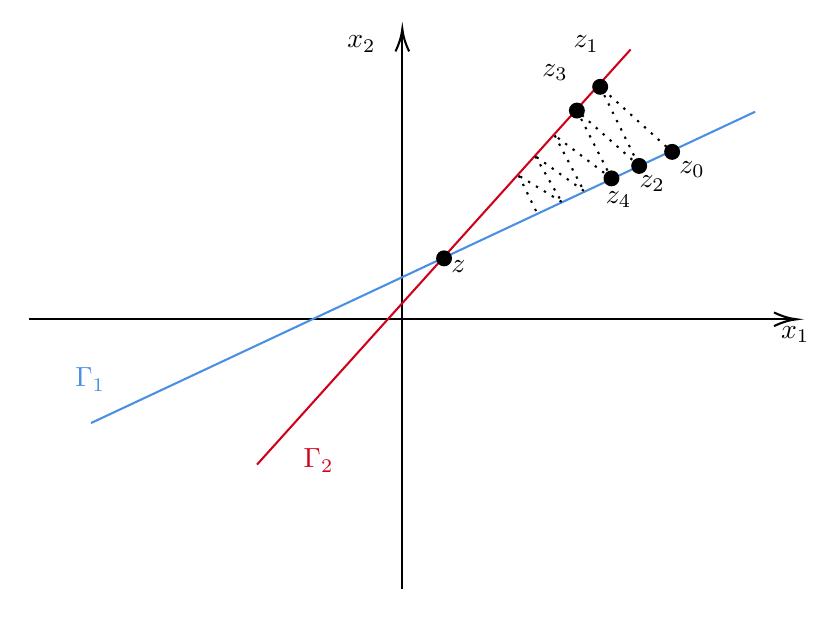
\begin{tikzpicture}[x=0.75pt,y=0.75pt,yscale=-1,xscale=1]
%uncomment if require: \path (0,300); %set diagram left start at 0, and has height of 300

%Straight Lines [id:da75457235464343] 
\draw    (270,280) -- (270,12) ;
\draw [shift={(270,10)}, rotate = 450] [color={rgb, 255:red, 0; green, 0; blue, 0 }  ][line width=0.75]    (10.93,-3.29) .. controls (6.95,-1.4) and (3.31,-0.3) .. (0,0) .. controls (3.31,0.3) and (6.95,1.4) .. (10.93,3.29)   ;
%Straight Lines [id:da7722085314773515] 
\draw    (90,150) -- (458,150) ;
\draw [shift={(460,150)}, rotate = 180] [color={rgb, 255:red, 0; green, 0; blue, 0 }  ][line width=0.75]    (10.93,-3.29) .. controls (6.95,-1.4) and (3.31,-0.3) .. (0,0) .. controls (3.31,0.3) and (6.95,1.4) .. (10.93,3.29)   ;
%Straight Lines [id:da3699929680974503] 
\draw [color={rgb, 255:red, 74; green, 144; blue, 226 }  ,draw opacity=1 ]   (440,50) -- (120,200) ;
%Straight Lines [id:da7625021948985371] 
\draw [color={rgb, 255:red, 208; green, 2; blue, 27 }  ,draw opacity=1 ]   (380,20) -- (200,220) ;
%Flowchart: Connector [id:dp6701639386639788] 
\draw  [fill={rgb, 255:red, 0; green, 0; blue, 0 }  ,fill opacity=1 ] (396.67,69.33) .. controls (396.67,67.49) and (398.16,66) .. (400,66) .. controls (401.84,66) and (403.33,67.49) .. (403.33,69.33) .. controls (403.33,71.17) and (401.84,72.67) .. (400,72.67) .. controls (398.16,72.67) and (396.67,71.17) .. (396.67,69.33) -- cycle ;
%Straight Lines [id:da9001208077053047] 
\draw  [dash pattern={on 0.84pt off 2.51pt}]  (400.56,69.89) -- (365.33,38) ;
%Flowchart: Connector [id:dp5225207453723415] 
\draw  [fill={rgb, 255:red, 0; green, 0; blue, 0 }  ,fill opacity=1 ] (362,38) .. controls (362,36.16) and (363.49,34.67) .. (365.33,34.67) .. controls (367.17,34.67) and (368.67,36.16) .. (368.67,38) .. controls (368.67,39.84) and (367.17,41.33) .. (365.33,41.33) .. controls (363.49,41.33) and (362,39.84) .. (362,38) -- cycle ;
%Straight Lines [id:da9929026232063627] 
\draw  [dash pattern={on 0.84pt off 2.51pt}]  (365.33,38) -- (384.11,76.11) ;
%Flowchart: Connector [id:dp6874731054911261] 
\draw  [fill={rgb, 255:red, 0; green, 0; blue, 0 }  ,fill opacity=1 ] (367.44,82.11) .. controls (367.44,80.27) and (368.94,78.78) .. (370.78,78.78) .. controls (372.62,78.78) and (374.11,80.27) .. (374.11,82.11) .. controls (374.11,83.95) and (372.62,85.44) .. (370.78,85.44) .. controls (368.94,85.44) and (367.44,83.95) .. (367.44,82.11) -- cycle ;
%Flowchart: Connector [id:dp4569133615919896] 
\draw  [fill={rgb, 255:red, 0; green, 0; blue, 0 }  ,fill opacity=1 ] (380.78,76.11) .. controls (380.78,74.27) and (382.27,72.78) .. (384.11,72.78) .. controls (385.95,72.78) and (387.44,74.27) .. (387.44,76.11) .. controls (387.44,77.95) and (385.95,79.44) .. (384.11,79.44) .. controls (382.27,79.44) and (380.78,77.95) .. (380.78,76.11) -- cycle ;
%Straight Lines [id:da7746684553332599] 
\draw  [dash pattern={on 0.84pt off 2.51pt}]  (384.11,76.11) -- (354.11,49.44) ;
%Flowchart: Connector [id:dp975033746659234] 
\draw  [fill={rgb, 255:red, 0; green, 0; blue, 0 }  ,fill opacity=1 ] (350.78,49.44) .. controls (350.78,47.6) and (352.27,46.11) .. (354.11,46.11) .. controls (355.95,46.11) and (357.44,47.6) .. (357.44,49.44) .. controls (357.44,51.29) and (355.95,52.78) .. (354.11,52.78) .. controls (352.27,52.78) and (350.78,51.29) .. (350.78,49.44) -- cycle ;
%Straight Lines [id:da1444355411515561] 
\draw  [dash pattern={on 0.84pt off 2.51pt}]  (354.11,49.44) -- (370.78,82.11) ;
%Straight Lines [id:da13565184184925871] 
\draw  [dash pattern={on 0.84pt off 2.51pt}]  (370.78,82.11) -- (343.44,61.44) ;
%Straight Lines [id:da13425341749894493] 
\draw  [dash pattern={on 0.84pt off 2.51pt}]  (343.44,61.44) -- (357.44,88.11) ;
%Straight Lines [id:da6091299471794016] 
\draw  [dash pattern={on 0.84pt off 2.51pt}]  (357.44,88.11) -- (334.11,71.44) ;
%Straight Lines [id:da8168868507181868] 
\draw  [dash pattern={on 0.84pt off 2.51pt}]  (334.11,71.44) -- (346.78,93.44) ;
%Straight Lines [id:da22056627322376565] 
\draw  [dash pattern={on 0.84pt off 2.51pt}]  (346.78,93.44) -- (326.11,80.78) ;
%Straight Lines [id:da35087366344294124] 
\draw  [dash pattern={on 0.84pt off 2.51pt}]  (326.11,80.78) -- (334.87,98.73) ;
%Flowchart: Connector [id:dp04320124093495181] 
\draw  [fill={rgb, 255:red, 0; green, 0; blue, 0 }  ,fill opacity=1 ] (286.78,120.64) .. controls (286.78,118.8) and (288.27,117.31) .. (290.11,117.31) .. controls (291.95,117.31) and (293.44,118.8) .. (293.44,120.64) .. controls (293.44,122.49) and (291.95,123.98) .. (290.11,123.98) .. controls (288.27,123.98) and (286.78,122.49) .. (286.78,120.64) -- cycle ;

% Text Node
\draw (451,152) node [anchor=north west][inner sep=0.75pt]   [align=left] {$\displaystyle x_{1}$};
% Text Node
\draw (242,12) node [anchor=north west][inner sep=0.75pt]   [align=left] {$\displaystyle x_{2}$};
% Text Node
\draw (111,172) node [anchor=north west][inner sep=0.75pt]   [align=left] {$\displaystyle \textcolor[rgb]{0.29,0.56,0.89}{\Gamma _{1}}$};
% Text Node
\draw (221,211) node [anchor=north west][inner sep=0.75pt]   [align=left] {$\displaystyle \textcolor[rgb]{0.82,0.01,0.11}{\Gamma _{2}}$};
% Text Node
\draw (402,72.33) node [anchor=north west][inner sep=0.75pt]   [align=left] {$\displaystyle z_{0}$};
% Text Node
\draw (351,12) node [anchor=north west][inner sep=0.75pt]   [align=left] {$\displaystyle z_{1}$};
% Text Node
\draw (382.78,79.11) node [anchor=north west][inner sep=0.75pt]   [align=left] {$\displaystyle z_{2}$};
% Text Node
\draw (336,25.93) node [anchor=north west][inner sep=0.75pt]   [align=left] {$\displaystyle z_{3}$};
% Text Node
\draw (366.6,86.8) node [anchor=north west][inner sep=0.75pt]   [align=left] {$\displaystyle z_{4}$};
% Text Node
\draw (292.11,120.31) node [anchor=north west][inner sep=0.75pt]   [align=left] {$\displaystyle z$};


\end{tikzpicture}

    \label{fig:kach}
    \caption{Двумерный пример алгоритма Качмажа.}
\end{figure}

Для начала запишем систему уравнений используя скалярное произведение:
\[
    \begin{cases}
        (\vect{a_1},\, \vect{x})=\vect{b_1}, \\
        (\vect{a_2},\, \vect{x})=\vect{b_2}, \\
        \ldots                               \\
        (\vect{a_n},\, \vect{x})=\vect{b_n}. \\
    \end{cases}
\]

Можно заметить, что каждое уравнение задает гиперплоскость. Обозначим гиперплоскость, соответствующую
уравнению $(\vect{a_i},\, \vect{x})=\vect{b_i}$ как $\Gamma_i$. Тогда задачу можно переформулировать
следующим образом: \textit{найти пересечение гиперплоскостей $\Gamma=\Gamma_1\cap\Gamma_2\cap\ldots\cap\Gamma_n$}.

\begin{exercise}
    Рассмотрим пример:
    \[
        \begin{cases}
            a_{11}x_1+a_{12}x_2=b_1 \\
            a_{21}x_1+a_{22}x_2=b_2 \\
        \end{cases}
    \]

    Возьмем некоторую точку $z_0$ на одной из гиперплоскостей.
    Берем $z_1$ как проекцию $z_0$ на вторую гиперплоскость.
    Аналогично $z_2$~--- проекция $z_1$ на первую плоскость.
    Продолжаем процесс (см. рис. \ref{fig:kach}).
\end{exercise}

В общем случае все аналогично. Можно доказать следующее утверждение, которое
и доказывает корректность данного алгоритма.

\begin{claim}
    Если $\det A\neq 0$, то последовательность, построенная алгоритмом
    Качмажа~--- сходящаяся, более того, сходящаяся к решению системы.
\end{claim}

Если же пересечение $\Gamma$ всех гиперплоскостей не является точкой, то справедливо следующее:
\begin{claim}
    Построенная последовательность будет сходится к некоторой $z\in\Gamma$, более
    того $z$~--- ближайшая к $z_0$ точка.
\end{claim}

\subsubsection{Generalized minimal residual method.}

Рассмотрим подпространства: \[
    L_1\subset L_2\subset\ldots\subset L_n=\Cx^{n}.
\]

Строим последовательность точек: \[
    x_k=x_0+y_k,\quad y_k\in L_k,\quad x_k=\argmin_{x_k\in x+L_k}\|b-Ax_k\|.
\]

Понятно, что $x_n$ будет решением системы. Остается вопрос: \textit{какие $L_i$ взять?}.
Рассмотрим \[
    L_1=L(\vect{r_0}),\quad L_2=L(\vect{r_0},\, A\vect{r_0}),\,
    L_3=L(\vect{r_0},\, A\vect{r_0},\, A^2\vect{r_0}),\,\ldots,
\]
где $\vect{r_0}=\vect{b}-A\vect{x_0}$.

\begin{remark}
    Пространства вида \[L_k=L(\vect{r_0},\, A\vect{r_0},\, \ldots,\, A^{k-1}\vect{r_0})\]
    называются\mdef{пространствами Крылова}.
\end{remark}

\begin{remark}
    Метод называется также\mdef{Generalized minimal residual method (GMRES)}.
\end{remark}

\subsubsection{Другой алгоритм.}

Рассмотрим теперь эрмитовы положительно определенные матрицы:
\[
    A\in\Cx^{n\times n},\quad A^*=A>0.
\]

\begin{definition}
    Матрица $A$ называется\mdef{положительно определенной}, если
    \[\vect{x}^*A\vect{x}>0\quad \forall \vect{x}\neq \vect{0},\quad \vect{x}\in\Cx^n.\]
\end{definition}

\begin{claim}
    Любая положительно определенная матрица является эрмитовой.
\end{claim}
